\chapter{Model matematyczny}

\section{Równanie Eikonału}

\indent\indent Zmienna $\phi$ w równaniu Eikonału \ref{eq:eikonal} modeluje czas przybycia frontu fali propagującej od powierzchni brzegu. Prawa strona równania wskazuje na jednostkową prędkość tego frontu, tzn. istnieje pole prędkości o $|\textbf{U}|=1$, co oznacza, że wyznaczona wartość jest równa szukanej odległości $d$\footcite{Tucker}.

\indent Zmodyfikowana forma równania z jawnym laplasjanem, jak poniżej, jest zwana równaniem Hamiltona-Jacobiego

\begin{equation}
\textbf{U}\circ\nabla\phi = 1 + \Gamma(\phi)\nabla^2\phi
\label{eq:eikonal_2}
\end{equation}

\indent Rozwiązanie \ref{eq:eikonal_2}, w oparciu o początkowy rozkład wartości $\phi$, otrzymuje się w sposób iteracyjny.
\section{Równanie Poissona}
\indent\indent Przy założeniu, że $\textbf{U}=0$ oraz $\Gamma = 1$, równanie \ref{eq:eikonal_2} można sprowadzić do równania Poissona 

\begin{equation}
\nabla^2 \phi = -1 \iff \frac{\partial^2 \phi}{\partial x^2} + \frac{\partial^2 \phi}{\partial y^2} = -1
\label{eq:poisson_1}
\end{equation}

\noindent Wstawiając wartości otrzymanego rozwiązania $\phi$ do zależności


\begin{equation}
d = - \sqrt{\left(\frac{\partial\phi}{\partial x}\right)^2+\left(\frac{\partial\phi}{\partial y}\right)^2}+\sqrt{\left(\frac{\partial\phi}{\partial x}\right)^2+\left(\frac{\partial\phi}{\partial y}\right)^2+2\phi}
\label{eq:d_1}
\end{equation}

\noindent otrzymuje się poszukiwaną odległość od brzegu. Należy mieć na uwadze, że wyprowadzenie wzoru \ref{eq:d_1} wymaga przyjęcia nieskończonych współrzędnych poza kierunkiem normalnym do brzegu. Oznacza to, że rozwiązanie jest dokładne tylko blisko ściany. Nie stanowi to znaczącego problemu w modelach turbulencji, bowiem korzystają one tylko z wartości $d$ wyznaczonych blisko brzegu\footnote{A ściślej - maksymalnie do jednej trzeciej grubości warstwy przyściennej (\textbf{ibid.})}

\section{Transformacja siatki z przestrzeni fizycznej do obliczeniowej}

\indent\indent W ramach niniejszego projektu została wygenerowana strukturalna siatka obliczeniowa o topologii typu O (ang. \textit{O-grid topology}), charakteryzująca się tym, że każdy z jej rzędów ($v=const$) tworzy wokół profilu krzywą zamkniętą, natomiast druga rodzina krzywych ($u=const$) rozciąga się prostoliniowo od powierzchni profilu (rys.~\ref{fig:siatka_krzywoliniowa}). Krzywa $v = 0$ pokrywa się z obwiednią profilu (od punktu \textsf{a} do \textsf{a'}), a linie $u=0$ (węzły \textsf{a}~-~\textsf{c}) oraz $u=u_{max}$ (węzły \textsf{a'}~-~\textsf{c'}) tną siatkę w przestrzeni obliczeniowej. Wadą topologii typu O jest słaba jakość siatki w miejscu ostrej krawędzi spływu, co wpływa na poprawność rozwiązania w tym obszarze\footcite{Blazek, s. 359}\footnote{Należy mieć na uwadze, że dobranie powyższego typu siatki, oraz sam fakt jej generowania w programie, jest czynnością pomocniczą wobec celu niniejszego projektu i służy jedynie sprawdzeniu poprawności implementacji modelu matematycznego.}.

\begin{figure}[H]
	\centering
	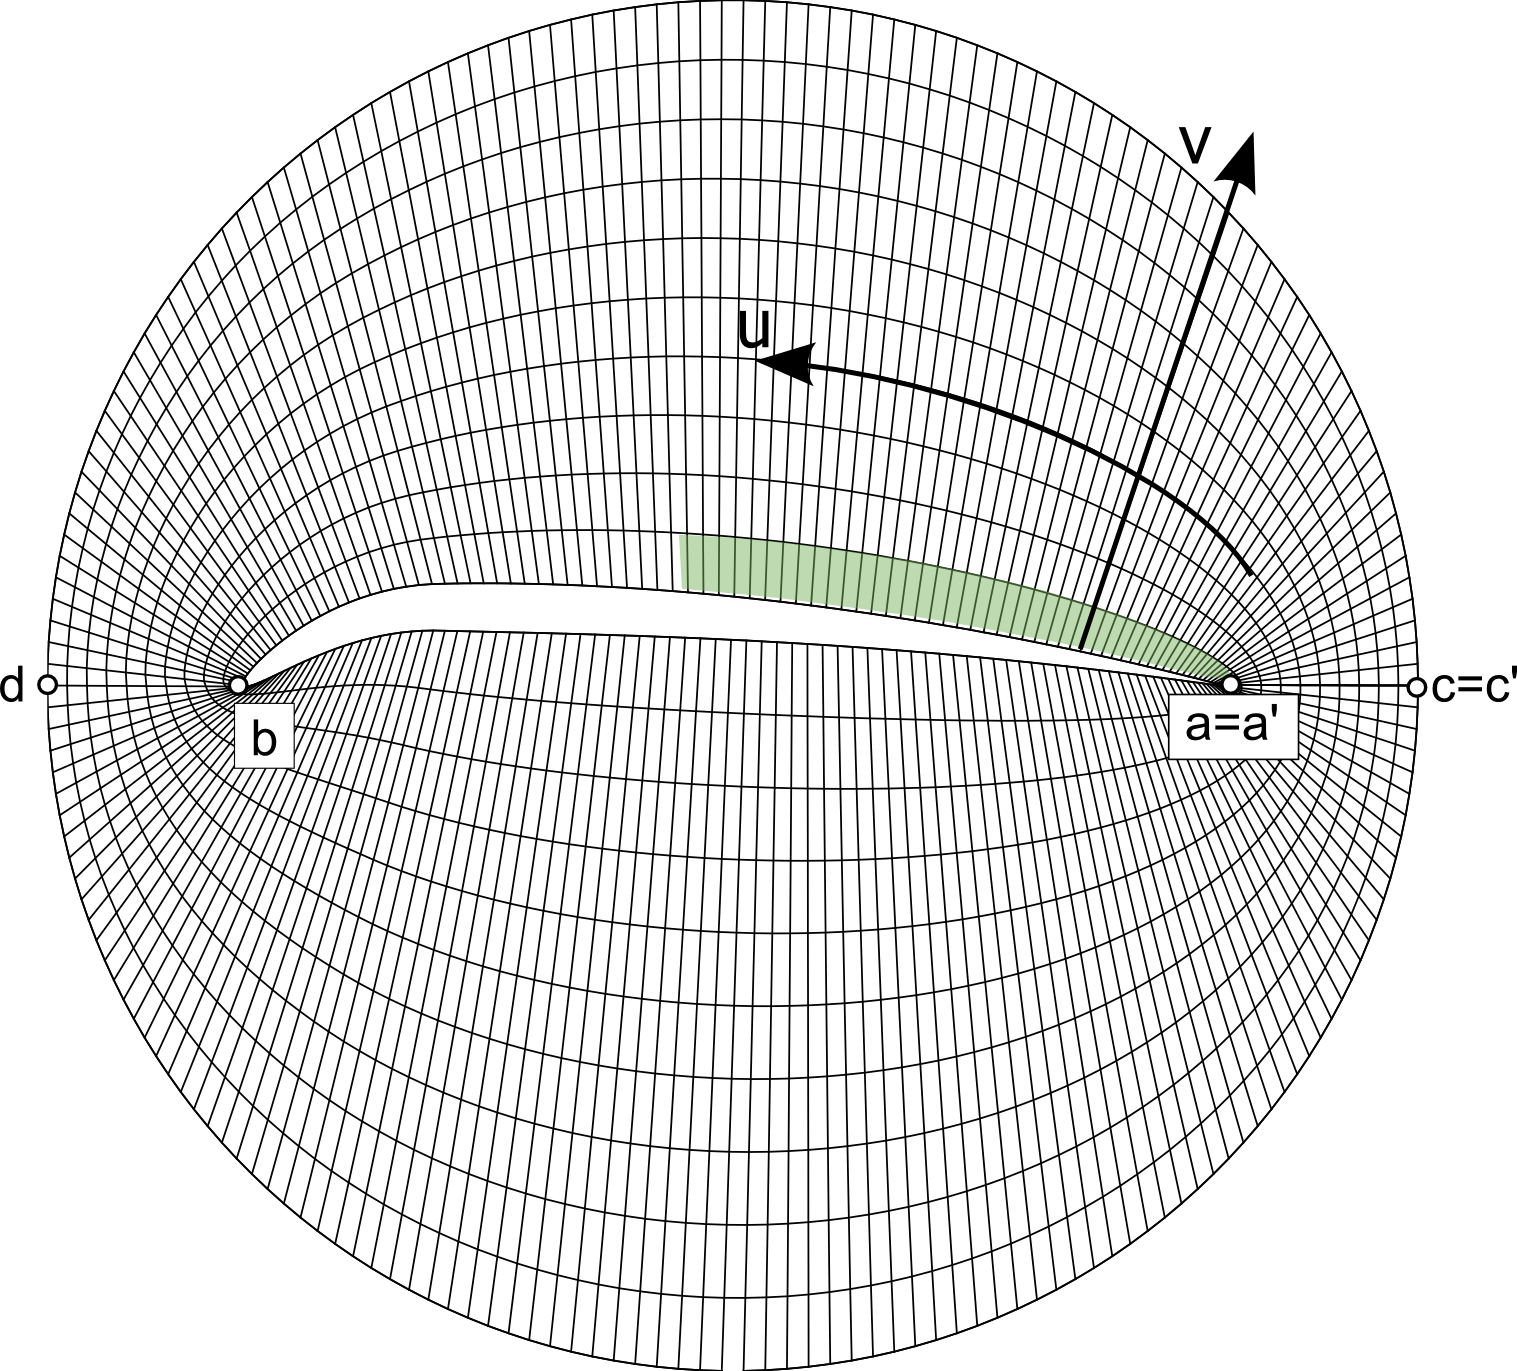
\includegraphics[width=0.8\linewidth]{Rysunki/siatka_krzywoliniowa.png}  
	\caption{Przestrzeń fizyczna. W oparciu o węzły leżące na konturze profilu została wygenerowana siatka krzywoliniowa o topologii O. Strzałkami oznaczono kierunki zmiennych $(u,v)$ z przestrzeni obliczeniowej. 
	\label{fig:siatka_krzywoliniowa}}
\end{figure} 

\begin{figure}[H]
	\centering
	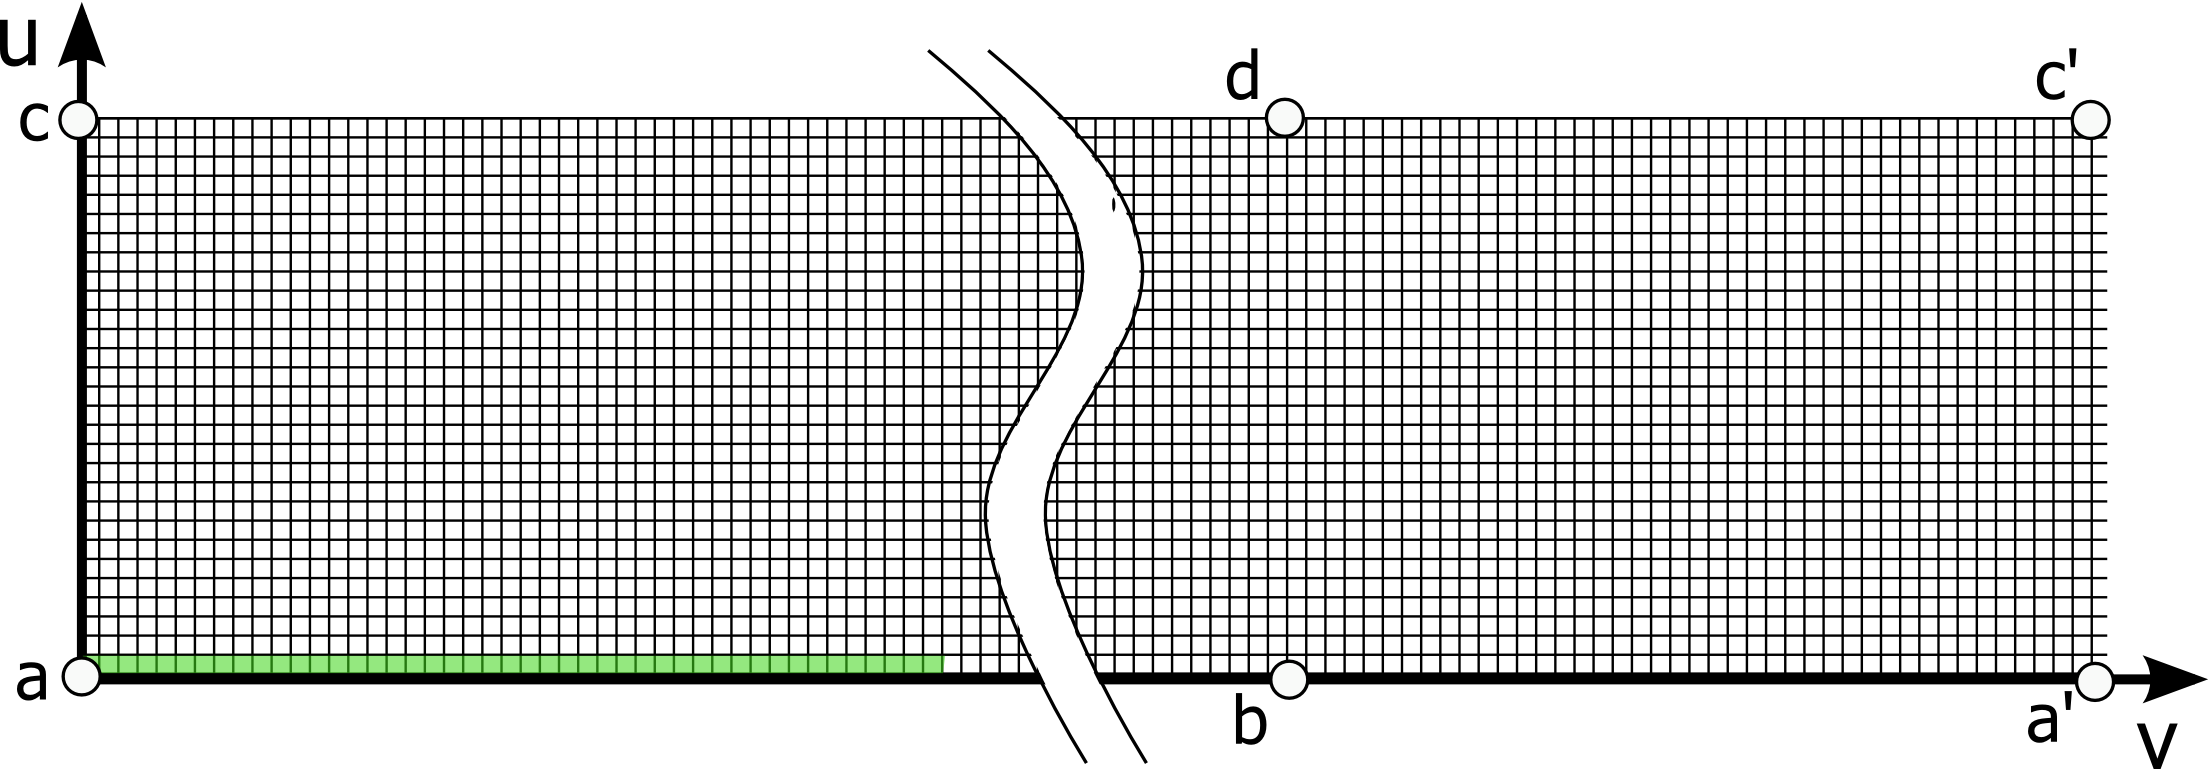
\includegraphics[width=\linewidth]{Rysunki/siatka_prostokatna.png}
	\caption{Przestrzeń obliczeniowa $(u,v)$. Węzły \textsf{a,a',b,c,c',d} odpowiadają węzłom z rys.~(\ref{fig:siatka_krzywoliniowa}). 
	\label{fig:siatka_obliczeniowa}}
\end{figure}

\indent Przyjętej w projekcie metody różnic skończonych nie da się bezpośrednio wykorzystać na siatce krzywoliniowej\footcite{Anderson, s. 170}. Wymagane jest przeprowadzenie transformacji siatki niejednorodnej do postaci prostokątnej, jak i samego równania Poissona, tak aby było spełnione w nowym układzie kartezjańskim (przekształcenie z przestrzeni fizycznej do obliczeniowej)\footcite{Blazek, s. 36}. 

\indent\newline Ogólna postać operatora laplasjanu we współrzędnych krzywoliniowych~$(u,v)$ wygląda  następująco\footnote{\url{http://www.maths.qmul.ac.uk/~wjs/MTH5102/curvcoord10.pdf}}

\begin{equation}
\nabla^2  = \frac{1}{h_1h_2}\left[\frac{\partial}{\partial u}\left(\frac{h_2}{h_1}\cdot\frac{\partial}{\partial u}\right)+\frac{\partial}{\partial v}\left(\frac{h_2}{h_1}\cdot\frac{\partial}{\partial v}\right) \right]
\end{equation}
\newline
\noindent Po wykonaniu różniczkowania wyrażeń w nawiasach okrągłych otrzymujemy jego rozwiniętą formę


\begin{equation} 
\begin{split}
\nabla^2
= 
\underbracket{\frac{1}{h_1^2}}_{A}\frac{\partial^2}{\partial u^2}
+ 
\underbracket{\frac{1}{h_2^2}}_{B}\frac{\partial^2}{\partial v^2}
& + 
\underbracket{\frac{1}{h_1h_2}\left[\frac{1}{h_1}\frac{\partial h_2}{\partial u} +  h_2\frac{\partial}{\partial u}\left(\frac{1}{h_1}\right) \right]}_{C}\frac{\partial}{\partial u}
 \\ & +
\underbracket{\frac{1}{h_1h_2}\left[ \frac{1}{h_2}\frac{\partial h_1}{\partial v}+h_1\frac{\partial}{\partial v}\left(\frac{1}{h_2}\right)\right]}_{D}\frac{\partial}{\partial v}
\end{split}
\label{eq:laplasjan_1}
\end{equation}

\noindent Występujące powyżej czynniki skalujące dane są następująco

\begin{equation}
h_1 = \sqrt{\left(\frac{\partial x}{\partial u}\right)^2+\left(\frac{\partial y}{\partial u}\right)^2}
\quad\quad\quad
h_2 = \sqrt{\left(\frac{\partial x}{\partial v}\right)^2+\left(\frac{\partial y}{\partial v}\right)^2}
\end{equation}
\newline
\noindent Pochodne czynników skalujących po współrzędnych obliczeniowych $u,v$ można wyrazić w postaci zależnej od współrzędnych z przestrzeni fizycznej $x,y$ 

\begin{equation}
\label{eq:poch_wsp_skal}
\begin{split}
\frac{\partial h_2}{\partial u} &= \frac{\partial}{\partial u}\left(\sqrt{x_v^2+y_v^2} \right)=\frac{x_v\cdot x_{uv}+y_v\cdot y_{vv}}{h_2} 
\\
\frac{\partial h_1}{\partial v} &= \frac{x_u\cdot x_{uv} + y_u\cdot y_{uv}}{h_1} 
\\
\frac{\partial}{\partial u}\left(\frac{1}{h_1}\right)&=\frac{\partial}{\partial u}\left(\frac{1}{\sqrt{x_u^2+y_u^2}}\right)= - \frac{x_u\cdot x_{uu} + y_u\cdot y_{uu}}{h_1^3}
\\
\frac{\partial}{\partial v}\left(\frac{1}{h_2}\right)&=-\frac{x_v\cdot x_{vv}+y_v\cdot y_{vv}}{h_2^3}
\end{split}
\end{equation}
\newline
\noindent Do obliczenia wartości poszczególnych pochodnych cząstkowych współrzędnych $x = x(u,v), y = y(u,v)$ po $u,v$ niezbędne jest użycie metody różnic skończonych.

\section{Dyskretyzacja metodą różnic skończonych}
\indent\indent W metodzie różnic skończonych operatory różniczkowania zastępowane są odpowiednimi operatorami różnicowymi. W rezultacie otrzymuje się układ równań algebraicznych, który w przeciwieństwie do układu równań różniczkowych jest prostszy i w większości przypadków w ogóle możliwy do rozwiązania. Otrzymany wynik jest jednak rozwiązaniem przybliżonym, o błędzie zależnym od wybranego rodzaju schematu różnicowego. Przybliżenie pochodnej różnicą centralną daje błąd o rząd mniejszy niż w przypadku różnicy w przód lub wstecznej, tzn. ma błąd obcięcia $\mathcal{O}(\Delta x)^2$. Fakt ten przemawia za użyciem jej w projekcie\footcite{Anderson, s. 132}.

\begin{figure}[H]
	\centering
    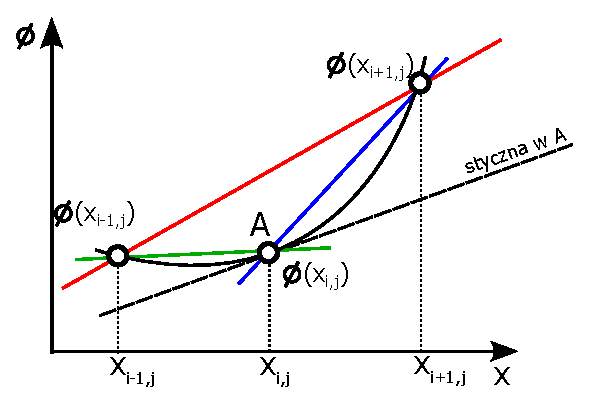
\includegraphics[width=0.6\linewidth]{Rysunki/roznice_skonczone_interpretacja.eps}
  \caption{Interpretacja geometryczna różnic skończonych: \color{blue}{przedniej}, \color{green}{wstecznej} \color{black}{oraz} \color{red}{centralnej} \color{black} wyraźnie wskazuje na przewagę tej ostatniej pod względem wielkości błędu popełnianego przy dyskretyzacji pochodnej.
	\label{fig:roznice_interpretacja}}
\end{figure}

\noindent Poniżej użyto oznaczeń $h_u, h_v$ na wartości kroku siatki odpowiednio na kierunku osi $Ou$ oraz $Ov$. \newline

\noindent Różnice dla pochodnych pierwszego rzędu:

\[
x_u = \frac{x_{i+1,j}-x_{i-1,j}}{2h_u} \quad\quad
 x_v = \frac{x_{i,j+1}-x_{i,j-1}}{2h_v}
\]

\begin{figure}[H]
	\centering
    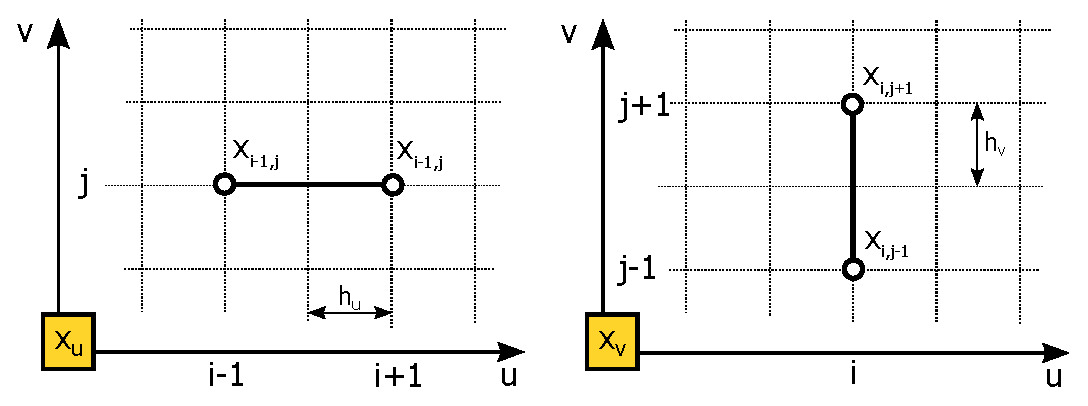
\includegraphics[width=\linewidth]{Rysunki/roznice_skonczone_x.eps}
	\caption{Konstrukcja różnic skończonych drugiego rzędu zmiennej \mbox{$x=x(u,v)$}
	\label{fig:roznice_skonczone_x}}
\end{figure}

\noindent Konstrukcja różnic dla $y_u, y_v$ jest analogiczna

\[
y_u = \frac{y_{i+1,j}-y_{i-1,j}}{2h_u} \quad y_v = \frac{y_{i,j+1}-y_{i,j-1}}{2h_v}
\]

\noindent Różnice dla pochodnych drugiego rzędu (rys.~\ref{fig:roznice_skonczone_xx}):

\[
x_{uu} = \frac{x_{i+1,j}-2x_{i,j}+x_{i-1,j}}{h_u^2} \quad x_{uv} = \frac{x_{i+1,j+1}-x_{i+1,j-1}-x_{i-1,j+1}+x_{x-1,j-1}}{4h_uh_v}
\]

\[
y_{uu} = \frac{y_{i+1,j}-2y_{i,j}+y_{i-1,j}}{h_u^2} \quad y_{uv} = \frac{y_{i+1,j+1}-y_{i+1,j-1}-y_{i-1,j+1}+y_{i-1,j-1}}{4h_uh_v}
\]


\begin{figure}[H]
	\centering
    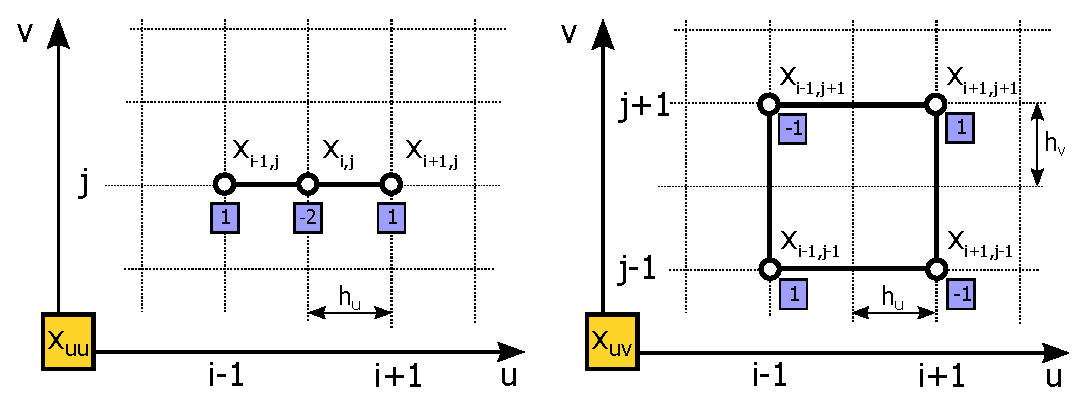
\includegraphics[width=\linewidth]{Rysunki/roznice_skonczone_xx.eps}
	\caption{Konstrukcja różnic skończonych drugiego rzędu dla zmiennej $x=x(u,v)$
	\label{fig:roznice_skonczone_xx}}
\end{figure}

\noindent Dla uproszczenia dalszego zapisu wprowadźmy następujące oznaczenie na wartość zmiennej $\phi$ w węźle o współrzędnych $(u_i,v_i)$:

\[
\phi(u_i, v_j) \triangleq \phi_{i,j}
\]

\noindent Wstawiając powyższe różnice do \ref{eq:poch_wsp_skal}, oraz analogicznie konstruując różnice dla zmiennej $\phi$, po wstawieniu otrzymanych związków do wzoru na laplasjan we współrzędnych obliczeniowych \ref{eq:laplasjan_1} otrzymujemy 
\begin{equation}
\begin{split}
A\cdot\frac{\phi_{i+1,j}-2\phi_{i,j}+\phi_{i-1,j}}{h_u^2}+B\cdot\frac{\phi_{i,j+1}-2\phi_{i,j}+\phi_{i,j-1}}{h_v^2}&+ \\ C\cdot\frac{\phi_{i+1,j}-\phi_{i-1,j}}{2h_v}+D\cdot\frac{\phi_{i,j+1}-\phi_{i,j-1}}{2h_v}&=-1
\end{split}
\end{equation}
\newpage \noindent Ostatecznie po uporządkowaniu względem $\phi$ równanie Poissona w postaci różnicowej wygląda następująco:
\begin{equation}
\begin{split}
\underbracket{\left(\frac{B}{h_v^2}-\frac{D}{2h_v}\right)}_{a}\phi_{i,j-1}\;&+\;\underbracket{\left(\frac{A}{h_u^2}-\frac{C}{2h_u}\right)}_{b}\phi_{i-1,j} \;\underbracket{-2\left(\frac{A}{h_u^2}+ 
\frac{B}{h_v^2}\right)}_{c}\phi_{i,j}\;+ \\ &+\; \underbracket{\left(\frac{A}{h_v^2} + \frac{C}{2h_u}\right)}_{d}\phi_{i+1,j}\;+\; \underbracket{\left(\frac{B}{h_v^2}+\frac{D}{2h_v}\right)}_{e}\phi_{i,j+1}=-1
\end{split}
\label{eq:poisson_roznicowo}
\end{equation}
\newline
\noindent Przedstawienie go w takiej formie umożliwia łatwe zapisanie układu równań dla całego obszaru obliczeniowego. Wzajemne rozmieszczenie przestrzenne węzłów odpowiadających poszczególnym wartościom zmiennej $\phi$, tworzących tzw. pięciopunktową gwiazdę różnicową (ang. \textit{five-point-star}), zaprezentowano na rys.~\ref{fig:wezly}.

\begin{figure}[h]
  \centering
    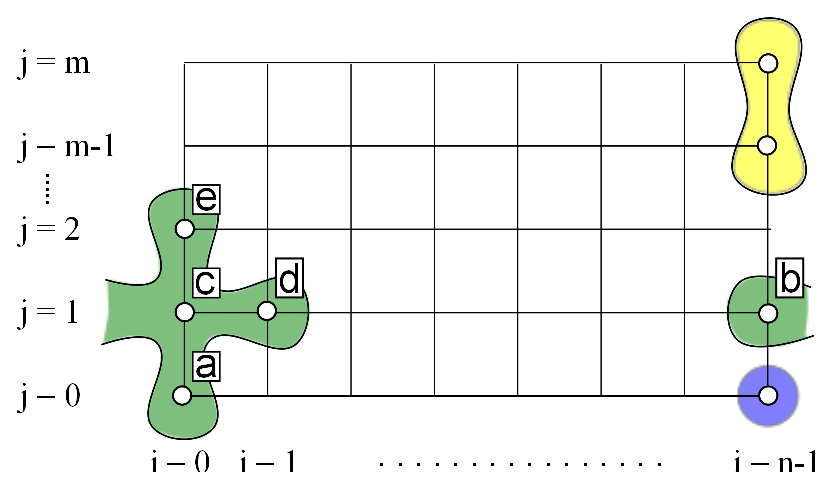
\includegraphics[scale=0.8]{Rysunki/gwiazda_roznicowa.eps}
  \caption{Siatka z wyróżnionymi węzłami, tworzącymi pięciopunktową \colorbox{green!70!blue!30}{gwiazdę różnicową} oraz warunki brzegowe: \colorbox{blue!30}{Dirichleta} i \colorbox{yellow!50}{Neumanna}.
  \label{fig:wezly}}
\end{figure}

\section{Warunki brzegowe}
\indent\indent Układ równań utworzony na podstawie wzoru \ref{eq:poisson_roznicowo} należy uzupełnić o poniższe warunki brzegowe (rys.~\ref{fig:wezly}).
\begin{enumerate}
\item \textbf{warunek ciągłości} - węzły leżące na lewej i prawej krawędzi siatki są w rzeczywistości węzłami sąsiadującymi ze sobą. W równaniu~\ref{eq:poisson_roznicowo} zapisanym dla węzła tego rodzaju wartość współczynnika \textsf{b} (lub odpowiednio~\textsf{d}) pochodzi z węzła leżącego na samym końcu (początku) tego samego rzędu siatki.
\item \textbf{warunek Dirichleta} - zerowa wartość zmiennej $\phi$ na krawędzi profilu
\begin{equation}
\phi\big|_{\partial S} = \phi_{i,0} = 0
\end{equation}
\item \textbf{warunek Neumanna} - zerowa wartość pochodnej $\phi$ w kierunku normalnym do zewnętrznego brzegu obszaru obliczeniowego \begin{equation}
\frac{\partial\phi}{\partial n}=0 \iff \frac{\phi_{i,m}-\phi_{i,m-1}}{h_v}=0
\end{equation}
gdzie: $m$ - indeks zewnętrznego rzędu siatki
\end{enumerate}

\section{Rozwiązanie zagadnienia}

\indent\indent Rozwiązanie uprzednio zdefiniowanego zagadnienia sprowadza się do rozwiązania macierzowego układu równań o postaci
\begin{equation}
\left[\mathbb{K}\right]\{\phi\}=\{f\}
\end{equation}
\noindent gdzie:
\begin{description}\addtolength{\itemsep}{-1.5\baselineskip}
  \item[\quad]$\mathbb{K}$ - macierz współczynników
  \item[\quad]$\{\phi\}$ - wektor poszukiwanych wartości funkcji $\phi$
  \item[\quad]$\{f\}$ - wektor prawej strony
\end{description}
\noindent W rozwiniętej formie równanie prezentuje się następująco (puste miejsca oznaczają zerowe elementy)

\begin{equation}
\begin{bmatrix}
      1 &   & 											\\[0.8pt]
        & 1 & 											\\[0.8pt]
        &   & \ddots 									\\[0.8pt]       
        &   &   & 1 									\\[0.8pt]           
      a &   &   &   & c & d &   & b & e 				\\[0.8pt]
        & a &   &   & b & c & d &   &   & e	    		\\[0.8pt]
        &&\ddots&&&\ddots&\ddots&\ddots&&&\ddots	   	\\[0.8pt]
        &   &   & a &   &   & b & c & d &   &   & e 	\\[0.8pt]
        &   &   &   & a & d &   & b & c &   &   &   & e \\[0.8pt]
        &   &   &   &   & -1&   &   &   & 1 &   &   &   \\[0.8pt]
        &   &   &   &   &   & -1&   &   &   & 1 &   &   \\[0.8pt]
        &   &   &   &   &   &  &\ddots &&   &&\ddots&   \\[0.8pt]
        &   &   &   &   &   &   &   & -1&   &   &   & 1 \\[0.8pt]
\end{bmatrix}
\begin{bmatrix}
	\phi_{0,0} 		\\[0.8pt]
	\phi_{1,0} 		\\[0.8pt]
		\vdots 		\\[0.8pt]
	\phi_{n-1,0} 	\\[0.8pt]
	\phi_{0,1} 		\\[0.8pt]
	\phi_{1,1} 		\\[0.8pt]
		\vdots 		\\[0.8pt]
	\phi_{n-2,1} 	\\[0.8pt]
	\phi_{n-1,1} 	\\[0.8pt]
	\phi_{0,m} 		\\[0.8pt]
	\phi_{1,m} 		\\[0.8pt]
		\vdots 		\\[0.8pt]
	\phi_{n-1,m}	\\[0.8pt]	
\end{bmatrix}
=
\begin{bmatrix}
	0 \\[0.8pt]
	0 \\[0.8pt]
	0 \\[0.8pt]
	0 \\[0.8pt]
   -1 \\[0.8pt]
   -1 \\[0.8pt]
   -1 \\[0.8pt]
   -1 \\[0.8pt]
   -1 \\[0.8pt]
   -1 \\[0.8pt]
	0 \\[0.8pt]
	0 \\[0.8pt]
	0 \\[0.8pt]
	0 \\[0.8pt]
\end{bmatrix}
\label{eq:poisson_macierz}
\end{equation}

\indent Macierz współczynników ma rozmiar $(n\cdot m)\times (n\cdot m)$, gdzie $n$ - liczba węzłów na profilu, $m$ - liczba rzędów siatki. Jej struktura jest charakterystyczna dla zagadnień opisanych równaniami różniczkowymi cząstkowymi, tzn. większość jej elementów jest  zerowa. Macierze o powyższej własności nazywane są rzadkimi (ang. \textit{sparse}) \footcite{Saad,s. 67}. Dla rozważanego w niniejszym projekcie problemu rozmiar macierzy wynosi $N\times N = 12\;524\times 12\;524 = 156\;850\;576$ elementów, z czego tylko $0{,}03\%$ ma niezerowe wartości\footnote{Macierz współczynników zawiera po $n$ wartości wynikających z warunków brzegowych Dirichleta i Neumanna, oraz $5n(m-2)$ z zapisu różnicowego równania Poissona. Procentowe wypełnienie macierzy można obliczyć następująco: $\frac{5n(m-2)+n+n}{n^2m^2}\approx\frac{5}{nm}$}. 

\indent Do rozwiązania układu \ref{eq:poisson_macierz} zdecydowano się na skorzystanie ze stabilizowanej metody wzajemnie sprzężonych gradientów BiCGSTAB (ang. \textit{BiConjugate Gradient STABilized method}). Jest to metoda iteracyjna, oparta na podprzestrzeniach Kryłowa, odpowiednia do zagadnień dobrze uwarunkowanych, z macierzami rzadkimi \footcite{Blazek,s. 208}. Za jej wykorzystaniem przemawia również dostępność implementacji w bibliotece Eigen (patrz podrozdział \ref{sec:bibl_zewn}).

\noindent Tolerancja rozwiązania została przyjęta na poziomie tolerancji danych wejściowych, tzn. $\epsilon = 10^{-6}$.




\indent W wyniku rozwiązania układu \ref{eq:poisson_macierz} otrzymuje się wartości $\phi$ wyrażone w przestrzeni obliczeniowej. Aby móc skorzystać ze wzoru na odległość~\ref{eq:d_1} należy rozwiązać pomocniczy układ równań wynikający wprost z reguły łańcuchowej \ref{eq:chain_rule}, mnożąc obie strony przez odwrotność macierzy Jacobiego.

\begin{equation}
\begin{cases}
	\phi_u = \phi_x\cdot x_u + \phi_y\cdot y_u \\
	\phi_v = \phi_x\cdot x_v + \phi_y\cdot y_v
\end{cases} \iff
\begin{bmatrix}
\phi_u \\ \phi_v
\end{bmatrix}=
\underbracket{\begin{bmatrix}
x_u && y_u \\
x_v && y_v
\end{bmatrix}}_{\text{macierz Jacobiego}}
\begin{bmatrix}
\phi_x \\ \phi_y
\end{bmatrix}
\label{eq:chain_rule}
\end{equation}

\begin{equation}
\begin{bmatrix}
\phi_x \\ \phi_y
\end{bmatrix} = 
\begin{bmatrix}
x_u && y_u \\
x_v && y_v
\end{bmatrix}^{-1}
\begin{bmatrix}
\phi_u \\ \phi_v
\end{bmatrix}
\label{eq:jakobian}
\end{equation}

\noindent\newline Szukana zależność transformacyjna \ref{eq:jakobian} wymaga dyskretyzacji pochodnych cząstkowych według przedstawionego wcześniej schematu różnicowego.

\[
\phi_u = \frac{\phi_{i+1,j}-\phi_{i-1,j}}{2h_u} \quad \phi_v = \frac{\phi_{i,j}-\phi_{i,j-1}}{h_v}
\]